\documentclass[10pt]{beamer}
\usetheme{Warsaw}
\usepackage[utf8]{inputenc}
\usepackage[english]{babel}
\usepackage{amsmath}
\usepackage{amsfonts}
\usepackage{amssymb}
\usepackage{wrapfig}
\usepackage{graphicx}
\usepackage{array}
\graphicspath{ {Images/} }
\author{
\footnotesize
\textbf{
\linebreak Achyuth Rao - 41056
\linebreak Akib Shaikh - 41062
\linebreak Arun Pottekat - 41054
\linebreak Pranav Tale - 41070
\linebreak 
\linebreak
Guide:- Prof. Mrs. Aparna Junnarkar
}
}

\title{
\small
\textbf{
Detection of DDoS in SDN environment using SVM and Entropy based mechanism.
}
}
\institute{

\includegraphics[width=2.75cm, height=2.9cm]{logo.png}\\ \textbf{PES's Modern College Of Engineering}} 
\date{}
\setbeamertemplate{footline}[frame number]{}
\setbeamertemplate{navigation symbols}{} 
\setbeamertemplate{caption}[numbered]
\setbeamertemplate{section in toc}[ball unnumbered]
\begin{document}

\begin{frame}
\titlepage
\end{frame}


\begin{frame}
\frametitle{Contents}
\footnotesize
\tableofcontents
\end{frame}



\begin{frame}

\frametitle{Introduction}
\section[]{Introduction}
\begin{itemize}
\footnotesize
\item
SDN separates intelligence from the hardware.
\item
SDN controller acts as network Operating System.
\item
This networking paradigm faces a lot of issues.
%\item
\item
DDoS attack makes the network resources unavailable.
\end{itemize}
\begin{figure}
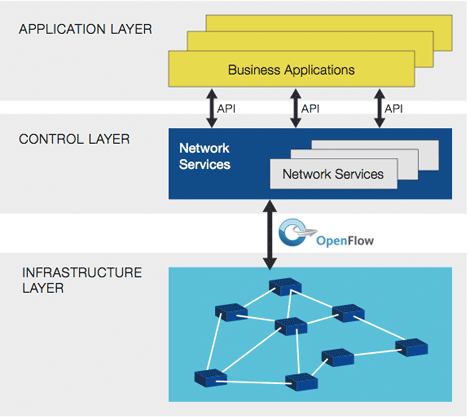
\includegraphics[scale=0.3]{SdnArchitecture.png}
\caption{\footnotesize SDN Architecture}
\end{figure}
\end{frame}






\begin{frame}
\section[]{Problem Statement}
\frametitle{Problem Statement}
\begin{itemize}
\footnotesize
\item
To provide a solution for the detection of DDoS attack in SDN environment using SVM and Entropy based mechanism and monitoring OpenFlow statistics.
\end{itemize}
\end{frame}




\begin{frame}
\section[]{Motivation}
\frametitle{Motivation}
\begin{center}
\begin{itemize}
\footnotesize
\item 
Number of cyber attacks is increasing day by day.
\item
Reluctance to adopt SDN due to lack of security solutions.
\item
A single DDoS attack can cost an enterprise over \$1.6 million.
\item
SDN market is expected to grow to \$56 Billion by 2022.
\item
Automation of attack detection is required.
\item
Integration of Machine Learning and Data Mining with SDN. 
\end{itemize}
\end{center}

\end{frame}



%\begin{frame}
% \frametitle{Literature Survey}
% \scriptsize
% \begin{center}
% \begin{tabular}{ | m{2cm} | m{2cm}| m{2cm} | m{3cm} | } 
% \hline
% \textbf{Title} & \textbf{Author} & \textbf{Journal and Year} & \textbf{Description} \\
% \hline
% DDoS Detection and Analysis in SDN-based Environment Using Support Vector Machine Classifier & 
% Kokila RT, S. Thamarai Selvi, Kannan Govindarajan & 
% IEEE 2014 & 
% This paper provides information about DDoS attack in SDN environment using Support Vector Machine to classify the attack.\\ 
% \hline
% An Entropy-Based Distributed DDoS Detection Mechanism in Software-Defined Networking &
% Rui Wang, Zhiping Jia, Lei Ju & 
% IEEE 2015 & 
% This paper provides information about DDoS attack in SDN environment using Entropy based mechanism to classify the attack.\\ 
% \hline
% Software-Defined Networking:The New Norm for Networks & 
% Open Networking Foundation & 
% ONF White Paper, 2012 & 
% Description about Software Defined Networks\\
% \hline
% Detection of DDoS Attacks using Enhanced Support Vector Machines with Real Time Generated Dataset & 
% T.Subbulakshmi, Dr. S. Mercy Shalinie, D. AnandK,  K.Kannatha&
% IEEE 2013 &
% Provided information how to create and use datasets for SVM.\\
% \hline
% OpenFlow Switch Specification& 
% Open Networking Foundation &
% Version 1.3.2 2013 &
% Description about OpenFlow Protocol\\
% \hline
% \end{tabular}
% \end{center}
% \end{frame}

\begin{frame}
\section[]{Objective}
\frametitle{Objective}
\begin{center}
\begin{itemize}
\footnotesize
\item
To apprehend different types of network attacks which can be launched on SDN.
\item
To compare different types of DDoS detection techniques.
\item
To propose the best effective method for a specific environment.
\item
To grasp an overview about the different network monitoring tools.
\end{itemize}
\end{center}
\end{frame}

\begin{frame}
\section[]{Scope}
\frametitle{Scope}
\begin{center}
\begin{itemize}
\footnotesize
\item
%OpenFlow protocol in SDN switches.
Set up of SDN environment.
\item
Entropy and SVM based DDoS detection method.
\item
OpenFlow Monitoring application using OpenDaylight API.
\end{itemize}
\end{center}
\end{frame}



%\begin{frame}
%\frametitle{Synopsis}
%\begin{center}
%\begin{itemize}
%\footnotesize
%\item
%SDN involves seperation of control and data plane.

%\item
%Security is a major concern in SDN architecture.

%\item
%DDoS attack results in exhaustion of controller resources.

%\item
%Entropy is a good measure of randomness.

%\item
%SVM is capable of decision making from uncertain information.

%\item
%Application for viewing OpenFlow statistics.
%\end{itemize}
%\end{center}
%\end{frame}


% \begin{frame}{
% \small
% \textbf{
% Scope
% }
% }
% \begin{itemize}
% \footnotesize
% \item
% Implementation of:
% \begin{itemize}
% \footnotesize
% \item
% Entropy mechanism.

% \item
% Support Vector Machine classifier.

% \item
% OpenFlow statistics monitoring application.
% \end{itemize}
% \end{itemize}
% \end{frame}

% \begin{frame}{
% \small
% \textbf{
% Architecture Diagram
% }
% }
% \begin{figure}[H]
% \includegraphics[scale=0.25]{Architecture_Diagram.png}
% \caption{
% System Architecture
% }
% \end{figure}
% \end{frame}


\begin{frame}
\section[]{Literature Survey}
\frametitle{Literature Survey}
\scriptsize
\begin{center}
\begin{tabular}{ | m{2cm} | m{2cm}| m{2cm} | m{3cm} | } 
\hline
\textbf{Title} & \textbf{Author} & \textbf{Journal and Year} & \textbf{Description} \\
\hline
DDoS Detection and Analysis in SDN-based Environment Using Support Vector Machine Classifier & 
Kokila RT, S. Thamarai Selvi, Kannan Govindarajan & 
IEEE 2014 & 
This paper provides information about DDoS attack in SDN environment using Support Vector Machine to classify the attack.\\ 
\hline
An Entropy-Based Distributed DDoS Detection Mechanism in Software-Defined Networking &
Rui Wang, Zhiping Jia, Lei Ju & 
IEEE 2015 & 
This paper provides information about DDoS attack in SDN environment using Entropy based mechanism to classify the attack.\\ 
\hline
Software-Defined Networking:The New Norm for Networks & 
Open Networking Foundation & 
ONF White Paper, 2012 & 
Description about Software Defined Networks\\
\hline
Detection of DDoS Attacks using Enhanced Support Vector Machines with Real Time Generated Dataset & 
T.Subbulakshmi, Dr. S. Mercy Shalinie, D. AnandK,  K.Kannatha&
IEEE 2013 &
Provided information how to create and use datasets for SVM.\\
\hline
OpenFlow Switch Specification& 
Open Networking Foundation &
Version 1.3.2 2013 &
Description about OpenFlow Protocol\\
\hline
\end{tabular}
\end{center}
\end{frame}



\begin{frame}
\section[]{Architecture Diagram}
\frametitle{Architecture Diagram}
\begin{figure}[H]
\includegraphics[scale=0.38]{myarch.png}
\caption{\footnotesize System Architecture}
\end{figure}
\end{frame}


\begin{frame}
\section[]{UML Diagrams}
\frametitle{UML Diagrams}
\begin{figure}
\includegraphics[scale=0.3]{use_case.png}
\caption{\footnotesize Use Case Diagram}
\end{figure}
\end{frame}

\begin{frame}
\frametitle{UML Diagrams}
\begin{figure}
\includegraphics[scale=0.35]{sequence.png}
\caption{\footnotesize Sequence Diagram}
\end{figure}
\end{frame}


\begin{frame}
\section[]{Mathematical Model}
\frametitle{Mathematical Model}
\footnotesize
$S = \lbrace \lbrace I \rbrace ,\lbrace P \rbrace ,\lbrace O \rbrace \rbrace $\newline\newline
$I = \lbrace N \rbrace$

\noindent
where,\\
$N = \lbrace $ Network Statistics $ \rbrace $, \\
$F =\lbrace F_{i} \mid F_{i} \in T , \forall i$ $ F_{i} =$ Individual entry $ \rbrace$, \\
$T = \lbrace $ Flow Table $ \rbrace$, \\
$F \subseteq N$
\newline

$P = \lbrace P_{EBD}, P_{SVM} \rbrace$
\newline

$O = \lbrace O_{EBD} \cup O_{SVM} \rbrace$

\end{frame}

\begin{frame}
\frametitle{Mathematical Model}
\footnotesize
$P_{EBD} $ $ (I_{EBD},$ $O_{EBD})$\\
$\lbrace$


\begin{itemize}
\footnotesize
\item $I_{EBD} = \lbrace U_{i} \mid U_{i} = ($ Src. Addr., Dest. Addr., Port no., Count$),  $ $ U_{i}  \subset F_{i} \rbrace$

\item $P_{i} = \frac{C_{i}}{N}$  

\item $\varepsilon = \sum_{i=0}^{n} - P_{i} log P_{i}$

\item $(\lambda < \varepsilon) \rightarrow  $ $ (\beta = 0)$ \\ $(\lambda > \varepsilon) \rightarrow  $ $ (\beta = 1)$

\item $ O_{EBD} = \lbrace \beta \mid \beta \in (0, $ $1) \rbrace$

\item $O_{EBD} = \lbrace z \mid \exists z, $ $ z \in \beta \rbrace$ \\

\end{itemize}
$ \rbrace$
\newline

$P_{SVM} $ $ (I_{SVM},$ $O_{SVM})$\\
$\lbrace$
\indent
\begin{itemize}
\footnotesize
\item $I_{SVM} = \lbrace V_{i} \mid V_{i} = ($ Src. Addr., Dest. Addr., Port no., Time, Prot., Count$) \rbrace$

\item $RBF = e^{-\gamma(\mid x_{1}-x_{2} \mid)+c}$ 

\item $y = \overline{\omega} * x + b$ 

\item $(y \leq -1) \rightarrow  $ $ (\alpha = 1)$ \\ $(y \geq 1) \rightarrow  $ $ (\alpha = 0)$

\item $ O_{SVM} = \lbrace \alpha \mid \alpha \in (0, $ $1) \rbrace$

\item $O_{SVM} = \lbrace x \mid \exists x, $ $ x \in \alpha \rbrace$ \\

\end{itemize}
$ \rbrace$

\end{frame}


\begin{frame}
\section[]{Algorithmic Strategies}
\frametitle{Algorithmic Strategies}
\begin{figure}
\includegraphics[scale=0.3]{SVM.png}
\caption{\footnotesize Flowchart: Support Vector Machine Algorithm}
\end{figure}
\end{frame}


\begin{frame}
\section[]{Algorithmic Strategies}
\frametitle{Algorithmic Strategies}
\begin{figure}
\includegraphics[scale=0.3]{EBD.png}
\caption{\footnotesize Flowchart: Entropy Based Discretization Mechanism}
\end{figure}
\end{frame}

	

\begin{frame}
\section[]{Software Specifications}
\frametitle{Software Specifications}
\begin{itemize}
\footnotesize
\item
Linux based Operating System.
\item
OpenDayLight Controller - 0.4.2 Berrylium SR2.
\item
Open vSwitch (OVS).
\item
PicOS / OpenSwitch.
\item
Oracle VirtualBox.
\item
Mininet 2.2.1.
\item
POX Controller.
\item
LibSVM.
\item
Python 2.7 or above.
\item
Nagios Core.
\item
NodeJS + AngularJS (JavaScript Framework). 
\end{itemize}
\end{frame}

\begin{frame}
\section[]{Hardware Specifications}
\frametitle{Hardware Specifications}
\begin{itemize}
\footnotesize
\item
Any Enterprise, Data Center, Campus Network Topology with 100/1000 Mbps.
\item
Switches that support OpenFlow Protocol / Whitebox Switches.
\begin{itemize}
\footnotesize
\item
HPE Altoline 6900 48G ONIE AC Switch.
\item
Pica8 P-3297 48 X 1Gbe.
\item
HP 2920 Switch Series.
\end{itemize}

\item
Server Running the Controller
\begin{itemize}
\footnotesize
\item
Dell PowerEdge R720
\end{itemize}

\end{itemize}
\end{frame}



\begin{frame}
\section[]{Dataset Specifications}
\frametitle{Dataset Specifications}
\begin{itemize}
\footnotesize
\item
"DDoS attack 2007" dataset provided by the Center for Applied Internet Data Analysis(CAIDA).
\item
The 1998 DARPA's network traffic dataset provided by MIT Lincoln Lab.
\item
The 2000 DARPA intrusion detection scenario specific dataset provided by MIT Lincoln Lab which contains:
\end{itemize}

\begin{table}
\scriptsize
\begin{center}
\begin{tabular}{ | m{2cm} | m{2cm}| m{2cm} |} 
\hline
\textbf{Data Category} & \textbf{No. of training instances} & \textbf{No. of test instances} \\
\hline
Break In &
156 &
374 \\
\hline
DDoS &
963 &
1035 \\
\hline
Installsw &
318 &
204 \\
\hline
IPSweep &
101 &
684 \\
\hline
Normal &
2500 &
2501 \\
\hline
Probe &
54 &
94 \\
\hline
Total &
4092 &
4892 \\
\hline
\end{tabular}
\end{center}
\caption{\footnotesize 2000 DARPA Dataset details}
\end{table}
\end{frame}


\begin{frame}
\section[]{Test Cases}
\frametitle{Test Cases}
\footnotesize
\begin{center}
\begin{tabular}{|p{0.5cm}|p{3.8cm}|p{2.2cm}|p{2.5cm}|}
\hline 
 \textbf{Id} & \textbf{Description} & \textbf{Scenario} & \textbf{Expected Output} \\ 
\hline 
 1 & Time span between attack detection and alert generation & Attack has occured & Instantaneous alert generation\\
 \hline
 2 & Normal Network Traffic, Log file not altered and attack is not detected & SDN functioning in normal mode & Alert not generated\\ 
\hline 
\end{tabular} 
\end{center}

\textbf{Scenario: Attack Traffic}
\begin{center}
\begin{tabular}{|p{0.5cm}|p{3.8cm}|p{2.2cm}|p{2.5cm}|}
\hline 
 \textbf{Id} & \textbf{Description} & \textbf{Input} & \textbf{Expected Output} \\ 
\hline 
 1 & Simple DoS attack & Large no. of same type of packets & Attack detected\\
 \hline
 2 & UDP flood attack & Large no. of UDP packets & Attack detected\\ 
 \hline
 3 & Varying DDoS attack bandwidth & Large no. of packets & DDoS attack should be detected only when bandwidth exceeds normal threshold traffic. \\
\hline 
\end{tabular} 
\end{center}
\end{frame}


\begin{frame}
\section[]{Results of Entropy Based Discretization}
\frametitle{Results of Entropy Based Discretization}
\begin{itemize}
\footnotesize
\item
Machine with Ubuntu 14.04, i5 CPU and 8G RAM.
\item
Mininet as a network simulator (Tree Topology, 800Mbps Link speed, 20 hosts).
\item
Open vSwitch.
\item 
Floodlight controller.
\item
CAIDA's "DDoS Attack 2007" dataset.
\end{itemize}
\scriptsize
\vspace{0.1cm}
\begin{table}
\begin{center}
\begin{tabular}{ | m{2cm} | m{2cm}| m{2cm} |} 
\hline
\textbf{S. No} & \textbf{Average Traffic Rate(Mbps)} & \textbf{Attack Rate(pkts/s)} \\
\hline
Exp.1 &
50 &
50-200 \\
\hline
Exp.2 &
100 &
300-500 \\ 
\hline
Exp.3 &
500 &
1000-2000 \\
\hline
\end{tabular}
\end{center}
\caption{parameter values of the Traffic}
\end{table}
\begin{figure}[h]
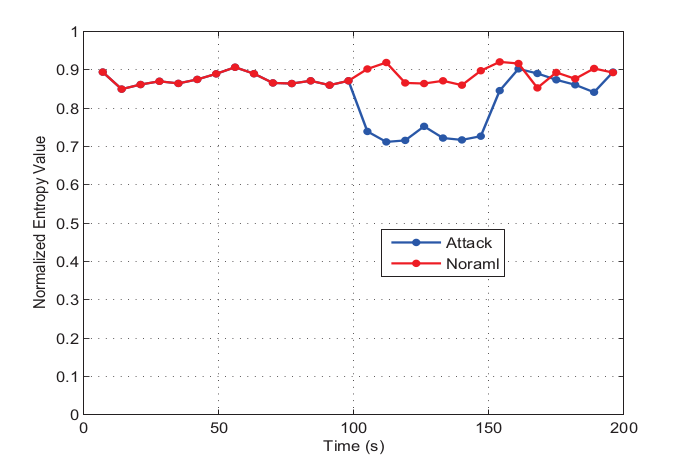
\includegraphics[scale=0.2]{Entropy.png}
\caption{\footnotesize The normalized entropy value of IPdst Flow}
\end{figure}

\end{frame}

\begin{frame}
\section[]{Results of SVM based Method}
\frametitle{Results of SVM based Method}

\begin{itemize}
\footnotesize
\item
%The 2000 DARPA intrusion detection scenario specific dataset %provided by MIT Lincoln lab is taken for evaluation.
The normal traffic data is included from 1998 DARPA dataset.
\item

The attack traffic data is included from 2000 DARPA dataset.
\end{itemize}

\begin{table}
\scriptsize
\begin{center}
\begin{tabular}{ | m{2cm} | m{2cm}| m{2cm} | m{2cm} |} 
\hline
\textbf{Cost} & \textbf{Gamma} & \textbf{Classification Accuracy(\%)} & \textbf{False Positive} \\
\hline
10 &
0.1 &
94.23 &
0.011 \\
\hline
10 &
0.01 &
95.11 &
0.008 \\
\hline
10 &
0.001 &
93.86 &
0.013 \\
\hline
\end{tabular}
\end{center}
\caption{\footnotesize Accuracy with different parameters}
\end{table}

\begin{figure}[h]
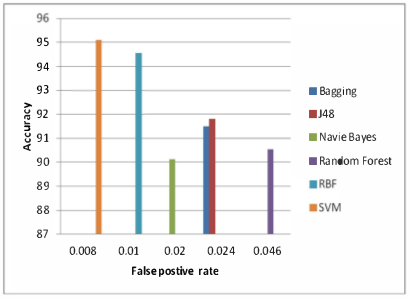
\includegraphics[scale=0.35]{svm.png}
\caption{Camparison of classification methods	}

\end{figure}
\end{frame}



\begin{frame}
\section[]{Conclusion}
\frametitle{Conclusion}

\begin{itemize}
\footnotesize
\item
Considering advantages and benefits delivered by SDN, its security issues need to be resolved.
\item
Thus this project is aimed at providing a solution for detection of DDoS attacks in SDN using Support Vector Machine and Entropy based discretization and evaluating the effectiveness of both the methods in a specific environment.
\end{itemize}
\end{frame}


\begin{frame}
\section[]{References}
\frametitle{References}
\begin{itemize}
\footnotesize
\item
"DDoS Detection and Analysis in SDN-based Environment Using Support Vector Machine Classifier" -Kokila RT, S. Thamarai Selvi, Kannan Govindarajan - 2014 Sixth International Conference on Advanced Computing(ICoAC) - Department of Computer Technology, Anna University (MIT Campus), Chennai.

\item
"An Entropy-Based Distributed DDoS Detection Mechanism in Software-Defined Networking" - Rui Wang, Zhiping Jia, Lei Ju - 2015 IEEE Trustcom/BigDataSE/ISPA - School of Computer Science and Technology Shandong University Jinan, China.

\item
"Software-Defined Networking:The New Norm for Networks and 
Open Networking Foundation" - Open Networking Foundation - ONF White Paper April 13, 2012.

\item
T.Subbulakshmi , Dr. S. Mercy Shalinie, V.GanapathiSubramanian, K.BalaKrishnan, D. AnandK, K.Kannathal - IEEE-ICoAC 2011 - Department of CSE, TCE Madurai, India.

\item
"OpenFlow Switch Specification" - Open Networking Foundation - Version 1.3.2 2013.

\end{itemize}
\end{frame}

\begin{frame}{}
\Huge
Thank You\ldots
\end{frame}
\end{document}